\documentclass[conference]{IEEEtran}

\usepackage{amsmath}
\usepackage{graphicx}
\usepackage{caption}
\usepackage{refstyle}
\usepackage{hyperref}

\graphicspath{{images/}}

\ifCLASSINFOpdf
 
\else
 
\fi

\hyphenation{op-tical net-works semi-conduc-tor}

\begin{document}

\title{Introdiction to Clustering with \\Gaussian Mixture Models and K-means}

\author{\IEEEauthorblockN{Esteban Guillen}
\IEEEauthorblockA{Computer Science\\
University of New Mexico\\
Albuquerque, NM 87131, USA\\
ejguill@unm.edu}}

\maketitle

\begin{abstract}
We live in a time when the amount of data being generated is growing at an incredible rate.  To better understand this vast amount of data we need automated methods to gain insight from the data.  This work introduces the Gaussian Mixture Model and two versions of the K-means algorithm.  The algorithms are compared on their computational performance and how quickly they converge to a solution.
\end{abstract}


\IEEEpeerreviewmaketitle




\section{Introduction}
Machine learning techniques provide a way to learn from data in an automated way.  Broadly speaking machine learning is often grouped into two categories, supervised learning and unsupervised learning.  Supervised learning involves training a model with data that has known answers (labels).  For example if we had a set of images that each contained a numerical digit and we knew (by filename or directory name) what digit each image depicted, then we could train a supervised learning algorithm to predict what digit a previously unseen image contained.  The key  idea for supervised learning is knowing the answers at training time.  While supervised learning approaches are successful in practice and there are many algorithms to choose from they have a fundamental limitation in that they need to know the answers at training time, which can required  many hours of intensive labor by humans.  Most of the data that exists today is unlabeled; the answers or categories are not know.  Unsupervised learning is designed to handle this unlabeled data.  

Clustering is a popular unsupervised learning technique and can broken down to two broad categories; hierarchical and partitioning.  This paper will focus on partitioning which seeks to group n objects into k clusters.  The Gaussian Mixture Model and K-means partitioning algorithms will be introduced through a series of experiments.  
\section{Background}

\subsection{K-means (Euclidean) }
Introduce Linear Regression
Show diagram the
Derive equations work
Introduce Linear Regression
Show diagram
Derive equations



\begin{equation}
\label{eqn_example}
x = \sum\limits_{i=0}^{z} 2^{i}Q
\end{equation}

\subsection{Gaussian Mixture Model with Expectation Maximization}
Introduce the need for regularization (penalize for complexity)
Derive equations my
Introduce Linear Regression
Show diagram hello
Derive equations work
Introduce Linear Regression
Show diagram
Derive equations

\subsection{K-means (Mahalanobis)}
Introduce Bayes' learning
Show diagram work
Derive equations
Introduce Bayes' learning
Show diagram
Derive equations
Introduce Bayes' learning
Derive equations
Introduce Bayes' learning
Show diagram hello
Derive equations
Introduce Bayes' learning my
Show diagram
Derive equations the
Introduce Bayes' learning
Show diagram
Derive equations


\section{Experiments}

A series of three experiments will introduce the reader to Gaussian Mixture Models and K-means. The first experiment will visualize the convergence of the algorithms for a fixed number of iterations, the second experiment will propose two methods for terminating the algorithms before reaching a maximum number of iterations, and the final experiment will show how to approximate the optimal number of clusters to use for running the algorithms.

\subsection{Data Sets}

\subsubsection{Data Set 1}
consists of 400 samples drawn randomly from 3 bivariate Gaussian distributions.  The 3 distributions are characterized by:

$$
\mu_1 = 
\begin{bmatrix} 
1 & 3  
\end{bmatrix}
\quad
\Sigma_1 = 
\begin{bmatrix} 
3 & 1  \\
1 & 2
\end{bmatrix}
$$

$$
\mu_2 = 
\begin{bmatrix} 
-1 & -2  
\end{bmatrix}
\quad
\Sigma_2 = 
\begin{bmatrix} 
2 & 0  \\
0 & 1
\end{bmatrix}
$$

$$
\mu_3 = 
\begin{bmatrix} 
3 & -3  
\end{bmatrix}
\quad
\Sigma_3 = 
\begin{bmatrix} 
1 & .3  \\
.3 & 1
\end{bmatrix}
$$

\subsubsection{Data Set 2}
 consists of 600 samples drawn randomly from 3 bivariate Gaussian distributions.  The 3 distributions are characterized by:

$$
\mu_1 = 
\begin{bmatrix} 
0 & 0  
\end{bmatrix}
\quad
\Sigma_1 = 
\begin{bmatrix} 
1 & -.9  \\
-.9 & 1
\end{bmatrix}
$$

$$
\mu_2 = 
\begin{bmatrix} 
-3 & -3.5  
\end{bmatrix}
\quad
\Sigma_2 = 
\begin{bmatrix} 
1 & .9  \\
.9 & 1
\end{bmatrix}
$$

$$
\mu_3 = 
\begin{bmatrix} 
3 & 2  
\end{bmatrix}
\quad
\Sigma_3 = 
\begin{bmatrix} 
1 & .9  \\
.9 & 1
\end{bmatrix}
$$

\subsubsection{Data Set 3}
consists of 600 samples drawn randomly from 3 bivariate Gaussian distributions.  The 3 distributions are characterized by:

$$
\mu_1 = 
\begin{bmatrix} 
-3 & 3  
\end{bmatrix}
\quad
\Sigma_1 = 
\begin{bmatrix} 
1 & 0  \\
0 & 1
\end{bmatrix}
$$

$$
\mu_2 = 
\begin{bmatrix} 
-3 & -3  
\end{bmatrix}
\quad
\Sigma_2 = 
\begin{bmatrix} 
1 & 0  \\
0 & 1
\end{bmatrix}
$$

$$
\mu_3 = 
\begin{bmatrix} 
4 & 0  
\end{bmatrix}
\quad
\Sigma_3 = 
\begin{bmatrix} 
1 & 0  \\
0 & 1
\end{bmatrix}
$$



\subsection{Experiment 1: Visualizing Convergence}
In this experiment the convergence for Gaussian Mixture Models, K-means (Euclidean), and K-means (Mahalanobis) is observed for data set 1.  Each algorithm is iterative and executes for 100 iterations during each run.  At the start of each run a random set (k=3) of $\mu_i$ vectors and $\Sigma_i$ matrices are used to initialize the 3 algorithms (K-means (Euclidean) only used the $\mu$ vectors).  30 restarts were used to increase the odds of finding a global optimum result for each algorithm.  The final convergence value for each algorithm was averaged over each restart for every iteration.  The Gaussian Mixture Model was evaluated using the log likelihood and the K-means algorithms were evaluated using their respective distance measures.  Results of the experiment are shown in Figures \ref{fig:ex_1a_log}, \ref{fig:ex_1a_maha}, and \ref{fig:ex_1a_eucl}.

 
\begin{figure}[h]
  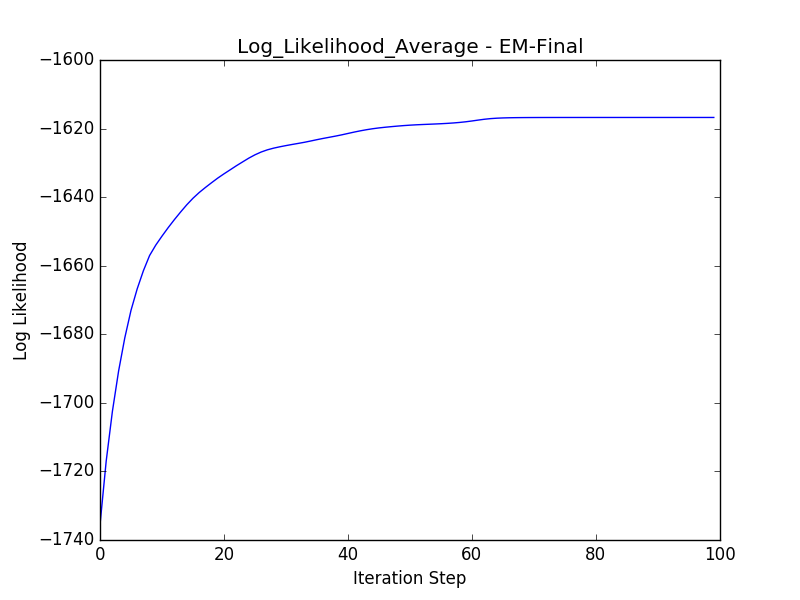
\includegraphics[width=0.5\textwidth]{experiment_1_log_likelihood_data1.png}
  \caption{The Average Log Likelihood from 30 Restarts for each Iteration}
  \label{fig:ex_1a_log}
\end{figure}

\begin{figure}[h]
  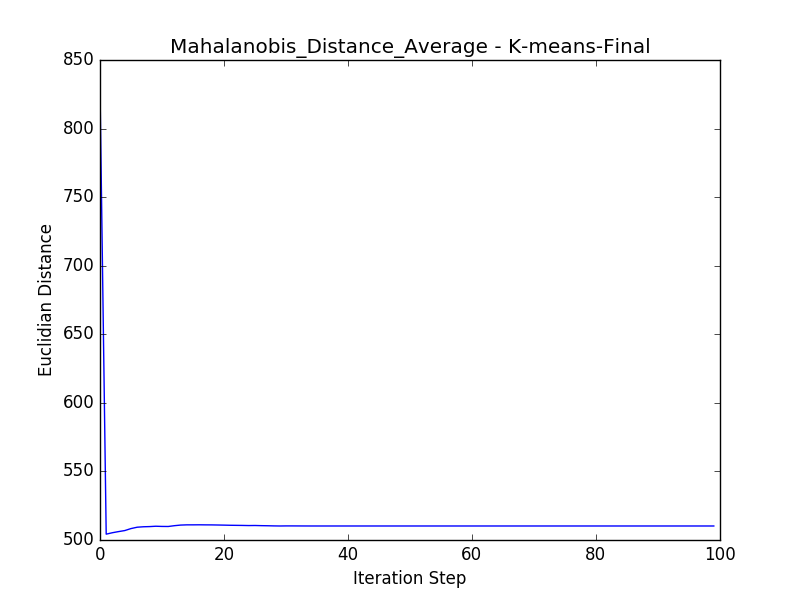
\includegraphics[width=0.5\textwidth]{experiment_1_mahalanobis_data1.png}
  \caption{The Average Mahalanobis Distance from 30 Restarts for each Iteration}
  \label{fig:ex_1a_maha}
\end{figure}

\begin{figure}[h]
  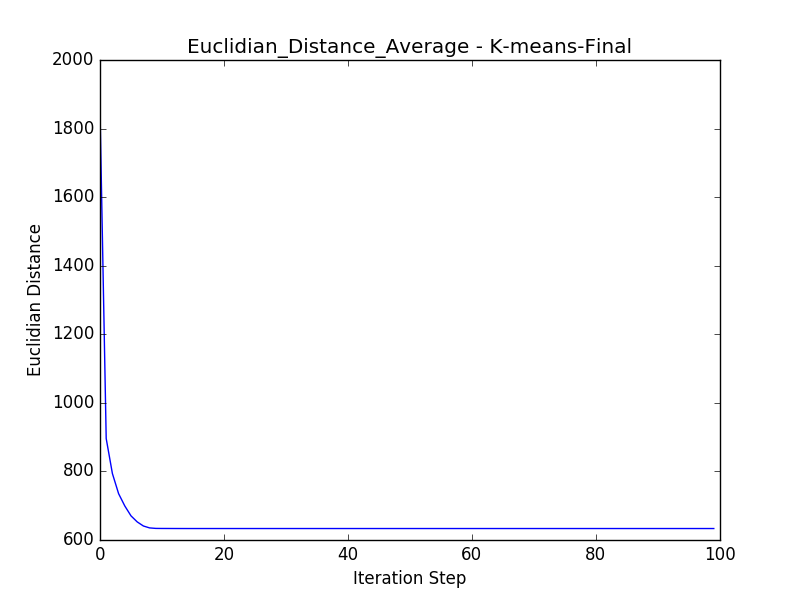
\includegraphics[width=0.5\textwidth]{experiment_1_euclidean_data1.png}
  \caption{The Average Euclidean Distance from 30 Restarts for each Iteration}
  \label{fig:ex_1a_eucl}
\end{figure}



\subsection{Experiment 2: Stopping Criteria}
In this experiment two different stopping criteria for Gaussian Mixture Models, K-means (Euclidean), and K-means (Mahalanobis) is observed for data set 1.

\subsection{Experiment 3: Finding the Optimal K}
Subsubsection text here.

\section{Discussion}
Explain the results of the experiments

\begin{table}[!t]
\renewcommand{\arraystretch}{1.3}
\caption{A Simple Example Table}
\label{table_example}
\centering
\begin{tabular}{c||c}
\hline
\bfseries First & \bfseries Next\\
\hline\hline
1.0 & 2.0\\
\hline
\end{tabular}
\end{table}

\section{Conclusion}
The conclusion goes here.  Summarize what was done summarize what was done, summarize what was done summarize what was done




\begin{thebibliography}{1}

\bibitem{IEEEhowto:kopka}
H.~Kopka and P.~W. Daly, \emph{A Guide to \LaTeX}, 3rd~ed.\hskip 1em plus
  0.5em minus 0.4em\relax Harlow, England: Addison-Wesley, 1999.
  
  
  

\end{thebibliography}





\end{document}


